\graphicspath{{figures_and_references/EELISA_conference/}}

% \selectlanguage{english}
\renewcommand{\chapternametext}{Chapter \thechapter: Introduction}

\chapter{\chapternametext}
\

\renewcommand{\headingtextL}{}
\renewcommand{\headingtextR}{\chapternametext}
\begingroup
 \flushbottom
 \setlength{\parskip}{0pt plus 1fil}%
 \localtableofcontents 
\endgroup

\begingroup
 \flushbottom
 \setlength{\parskip}{0pt plus 1fil}%
 \locallistoffigures
\endgroup


\newpage

\setcounter{section}{0} 



\FloatBarrier

\renewcommand{\sectionnametext}{Seismic risk in rapidly urbanizing and data-scarce regions}
\renewcommand{\headingtextL}{\chapternametext}
\renewcommand{\headingtextR}{\thesection. \sectionnametext}
\section{\sectionnametext}


Seismic risk in urban environments is defined by the interaction between geological hazards and the built environment. It is commonly expressed as the product of three interdependent components: hazard, exposure, and vulnerability. This relationship is formally written as:

\begin{center}
    \begin{math}
        Risk = Hazard \times Exposure \times Vulnerability
    \end{math}
\end{center}

In this formulation, \textbf{hazard} represents the physical occurrence of earthquakes and the associated ground motion characteristics, \textbf{exposure} describes the spatial distribution of buildings, infrastructure, and population, and \textbf{vulnerability} captures the likelihood that exposed assets will suffer damage under seismic loading conditions.

While seismic hazard modelling has reached a high level of scientific maturity, supported by decades of geophysical observation and probabilistic seismic hazard analysis, the same level of completeness does not exist for exposure and vulnerability modelling. These two components depend fundamentally on detailed knowledge of the built environment, including building geometry, construction materials, structural systems, and occupancy patterns. In practice, this information is rarely available in a consistent or up-to-date form.

This limitation becomes particularly critical in the context of global urbanization. Over the past decades, the majority of population growth has concentrated in urban areas, with a significant proportion occurring in developing countries. Cities in parts of Latin America, Africa, and Asia are expanding rapidly, often at rates that exceed the capacity of institutional planning systems. As a result, urban growth is frequently informal, spatially heterogeneous, and only partially documented in official records.

In high-income countries, seismic risk assessment is typically supported by comprehensive geospatial databases, cadastral systems, and engineering-grade building inventories. These datasets enable detailed exposure modelling at the level of individual structures, often including construction year, structural system, and compliance with seismic codes. However, in many developing regions, such datasets are either incomplete, outdated, or entirely absent. Municipal authorities may lack even a basic digital inventory of buildings, making systematic risk assessment extremely challenging.

This disparity creates a fundamental imbalance in global seismic resilience. Unfortunately, the regions that are often most exposed to high seismic hazard are also those with the least developed data infrastructure. Consequently, risk mitigation strategies in these areas are frequently reactive rather than proactive, relying on post-disaster assessments rather than continuous risk modelling.

Traditional approaches to addressing this gap have relied on field-based engineering surveys. These methods involve manual inspection of buildings by trained experts who classify structural systems, estimate material properties, and assess vulnerability based on observed characteristics. While these surveys are highly accurate and remain the gold standard for structural assessment, they are inherently limited in scalability. Conducting such surveys across entire metropolitan regions requires significant financial resources, time, and specialized personnel, making them impractical for large-scale or repeated assessments.

To address scalability constraints, remote sensing techniques have been increasingly adopted in recent years. Satellite imagery, aerial photography, and GIS-based data sources enable partial reconstruction of urban environments without direct physical access. These methods have proven effective for mapping urban extent, identifying general building footprints, and monitoring land-use changes over time. However, they typically operate at a level of abstraction that is insufficient for engineering applications. Most remote sensing approaches do not capture the structural detail required to distinguish between different building systems or to evaluate seismic vulnerability in a meaningful way.

This thesis is motivated by the need to bridge this gap. It proposes a computational framework capable of transforming raw geospatial observations into structured engineering knowledge. Rather than treating satellite imagery as a purely visual dataset, the proposed approach interprets it as a source of latent structural information that can be decoded using a combination of computer vision, machine learning, and physics-based modelling.

\renewcommand{\sectionnametext}{Scalable exposure models}
\renewcommand{\headingtextR}{\thesection. \sectionnametext}
\section{\sectionnametext}

The central challenge addressed in this research is the lack of scalable and reliable building exposure data in rapidly urbanizing regions. Buildings in these environments are often characterized by heterogeneous construction practices, informal development patterns, and limited enforcement of building regulations. This results in a built environment that is structurally diverse but poorly documented.

The absence of structured exposure data has direct implications for disaster risk reduction. Without knowledge of what is exposed, where it is located, and how it is constructed, it is impossible to accurately estimate seismic risk at meaningful spatial resolution. This limitation restricts the ability of governments and international organizations to prioritize interventions, allocate resources, or design effective mitigation strategies.

At the same time, advances in geospatial data availability and machine learning present new opportunities. High-resolution satellite imagery is now widely accessible, and foundational computer vision models have demonstrated strong generalization capabilities across domains. These developments open the possibility of reconstructing urban exposure layers even in the absence of formal cadastral data.

This thesis builds on recent advances in remote sensing, computer vision, and machine learning to propose a new paradigm for exposure modelling. In this paradigm, building inventories are not treated as static datasets but as dynamically inferred representations that integrate information from observable data, targeted field surveys, and insights derived from finite element models. By combining these sources of information, exposure models can be continuously updated and refined. At the same time, machine learning and computer vision models enable the generation of building-level predictions across entire urban areas, providing citywide coverage that would be impractical to achieve through field surveys alone.



\renewcommand{\sectionnametext}{From digital to hybrid twins}
\renewcommand{\headingtextR}{\thesection. \sectionnametext}
\section{\sectionnametext}


Traditional geospatial analysis has been largely descriptive, focusing on the representation of urban environments as static digital maps. In contrast, this thesis adopts a predictive and integrative approach, referred to as the \textbf{Hybrid Twin} paradigm.

A conventional Digital Twin is typically understood as a digital replica of a physical system. However, in the context of seismic risk assessment, such representations are insufficient because they lack predictive structural intelligence. The Hybrid Twin extends this concept by combining three complementary components:

\begin{itemize}
    \item \textbf{Observational Data:} Remote sensing imagery and geospatial datasets capturing the external geometry of urban environments.
    \item \textbf{Physics-Based Models:} Structural engineering principles that describe how buildings respond to seismic loading.
    \item \textbf{Data-Driven Models:} Machine learning systems capable of learning complex relationships between observed features and structural behavior.
\end{itemize}

By integrating these components, the Hybrid Twin becomes a dynamic system capable of inferring not only the geometry of urban environments, but also their structural and mechanical properties. This enables a transition from passive mapping to active risk modelling.

\renewcommand{\sectionnametext}{Integrating structural engineering aspects into geographic information systems}
\renewcommand{\headingtextR}{\thesection. \sectionnametext}
\section{\sectionnametext}

A central objective of this research is to move beyond conventional geographic information systems, which primarily describe the spatial distribution and geometry of the built environment. Instead, the proposed framework integrates structural engineering knowledge into geospatial modelling, enabling cities to be interpreted as collections of engineered structures whose properties can be inferred from data and governed by physical and construction-related constraints.

This integration supports a shift from purely descriptive spatial representation toward inference-based modelling, in which engineering-relevant attributes are derived from geospatial observations. These attributes include structural system typologies, plan and vertical irregularities, and seismic capacity curves. Although such properties are not directly observable in remote sensing imagery, they can be estimated by combining machine learning methods with structural engineering principles and physics-informed constraints.

The contribution of this work therefore extends beyond the automation of mapping and classification tasks. It establishes a framework for embedding structural interpretation within geospatial modelling, enabling the large-scale estimation of building-level structural characteristics for applications in seismic exposure modelling, risk assessment, and urban resilience analysis.


\renewcommand{\sectionnametext}{Objectives}
\renewcommand{\headingtextR}{\thesection. \sectionnametext}
\section{\sectionnametext}

The primary objectives of this thesis are:

\begin{enumerate}
    \item To develop scalable methods for automatic extraction of building footprints from remote sensing imagery.
    \item To formalize seismic codes into deterministic computational models.
    \item To infer structural characteristics of buildings using geospatial and visual proxies.
    \item To derive building-level seismic capacity curves that incorporate multiple behavioural modifiers without the need to explicitly simulate all possible combinations using finite element models.
    \item To integrate exposure, vulnerability, and hazard-related information into a unified computational framework.
    \item To develop a complete seismic vulnerability assessment workflow that is scalable, resolves building-level detail, is computationally efficient, and is suitable for application in developing regions.
\end{enumerate}


\renewcommand{\sectionnametext}{Research Highlights}
\renewcommand{\headingtextR}{\thesection. \sectionnametext}
\section{\sectionnametext}

\begin{figure}[htbp]
    \centering
    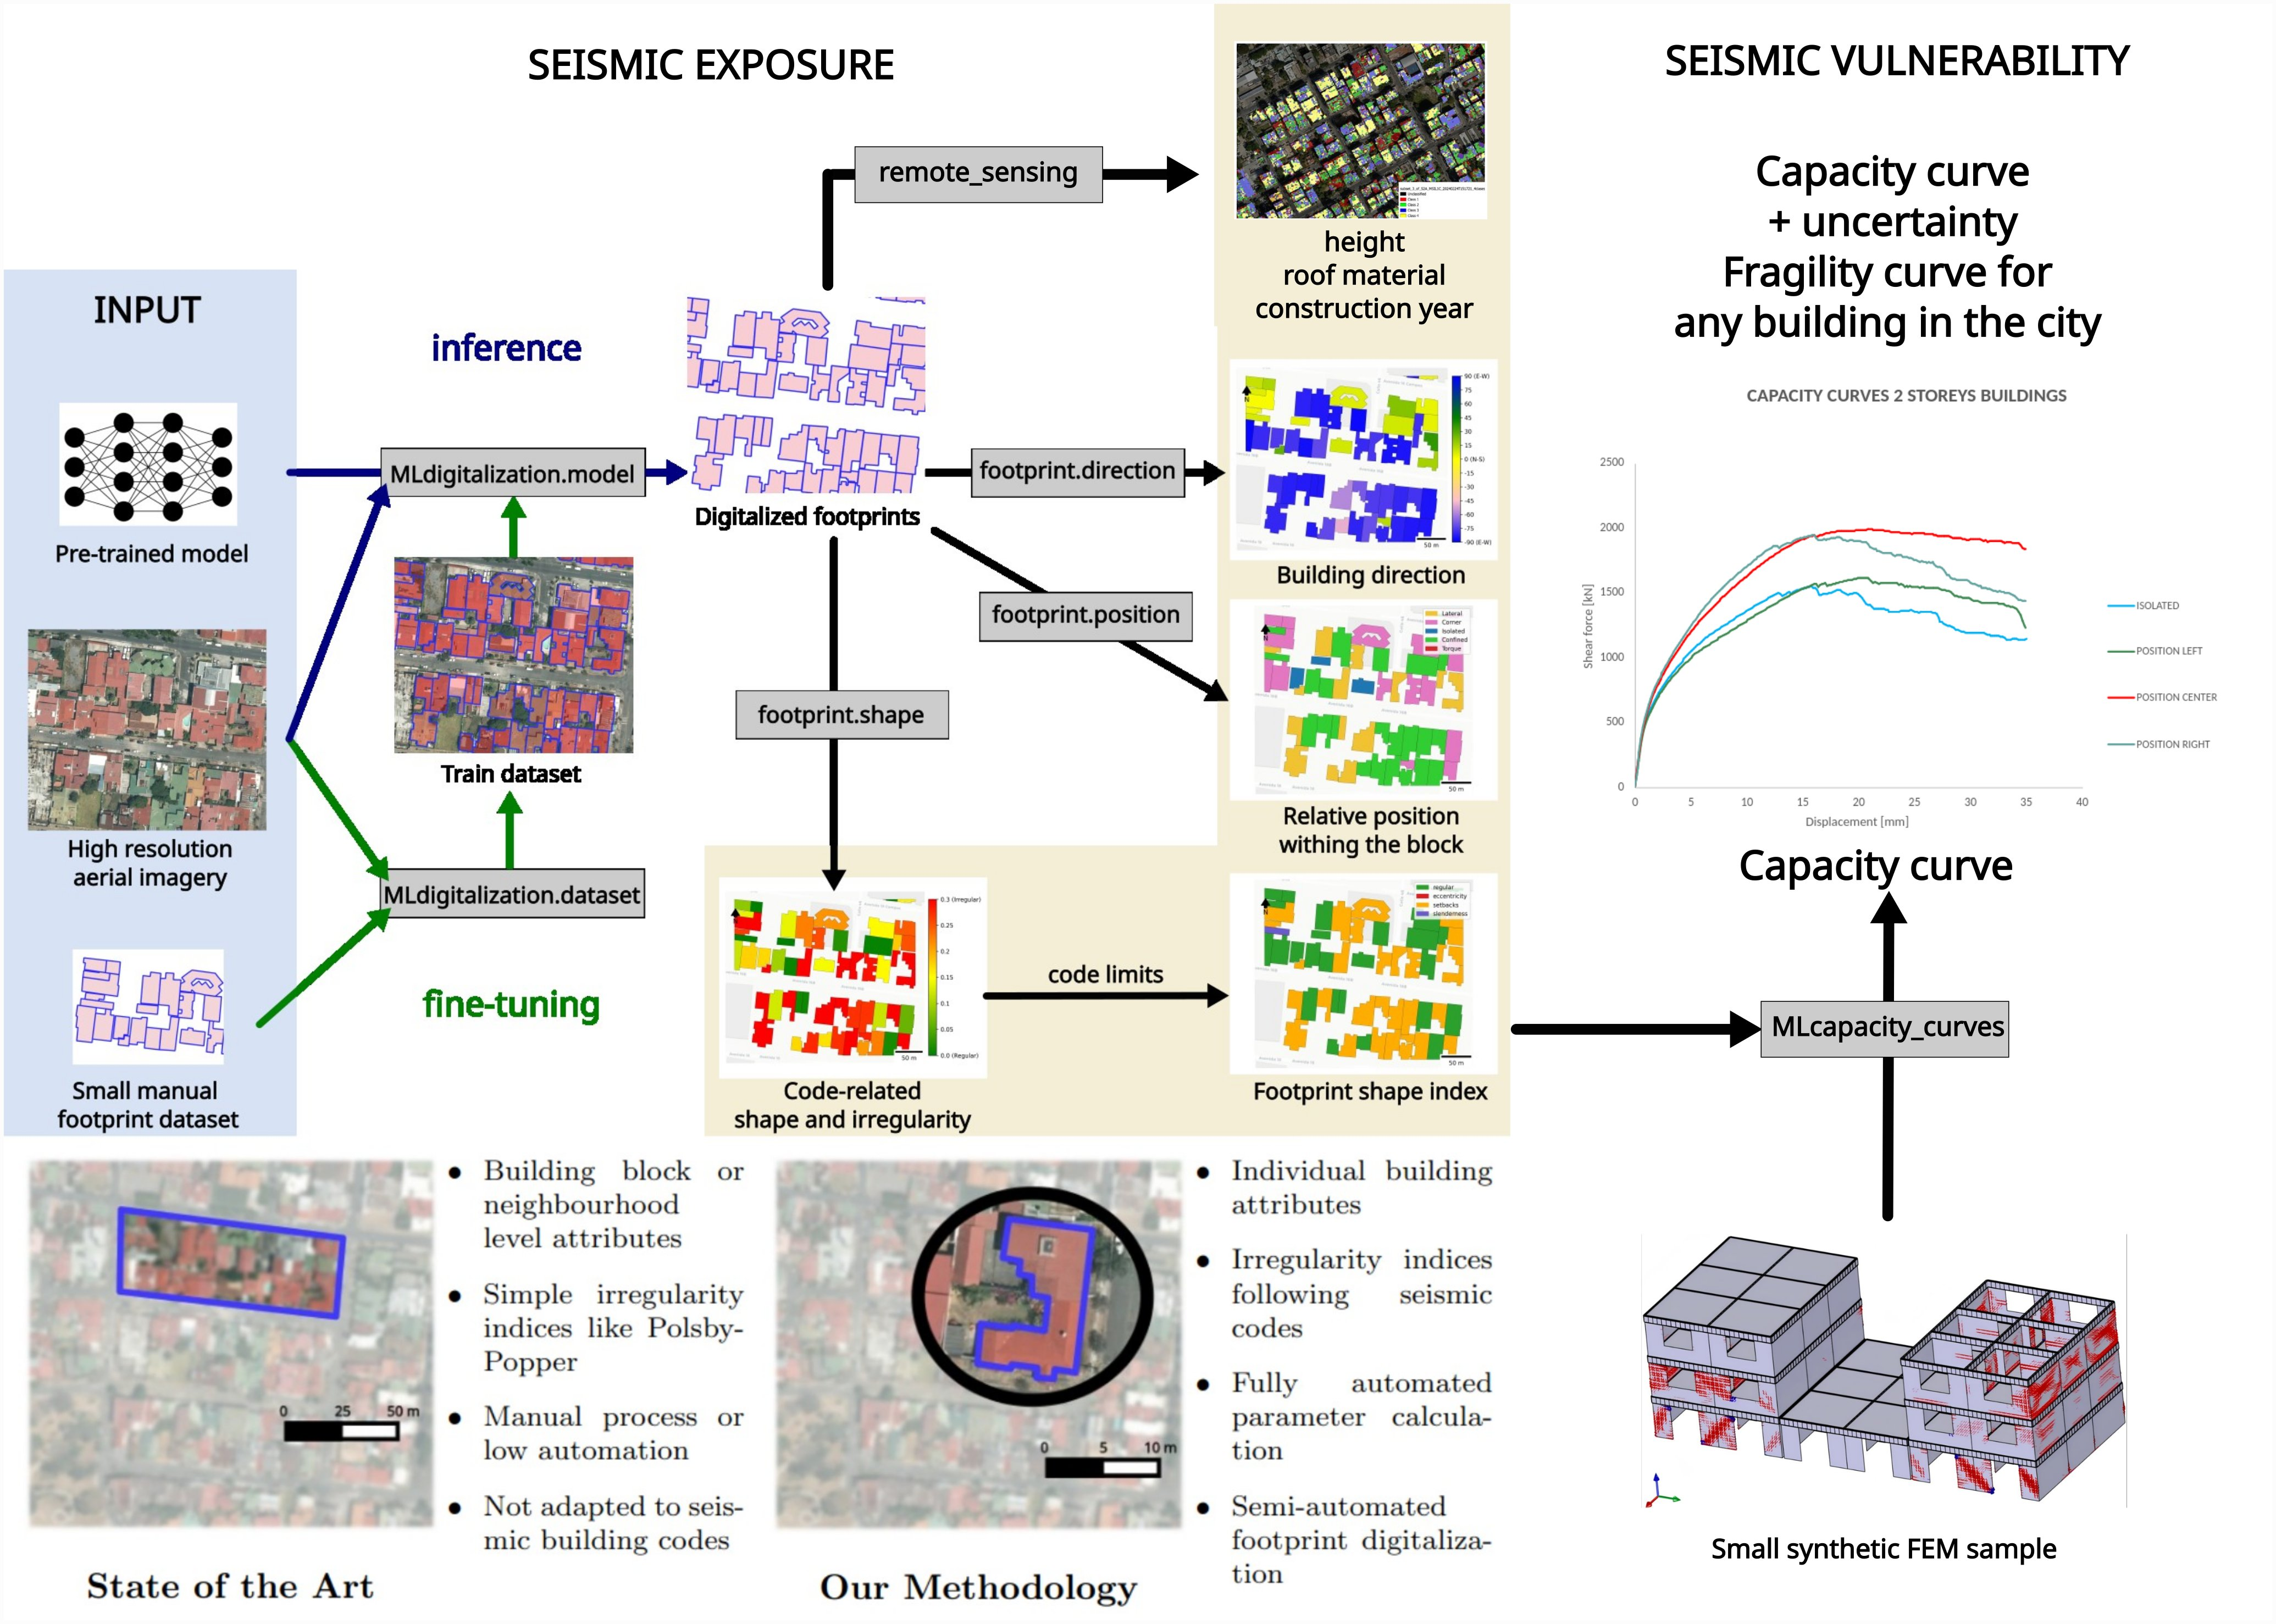
\includegraphics[width=\linewidth]{figures_and_references/complete_workflow.jpg}
    \caption{Complete proposed hybrid twin workflow.}
    \label{fig:complete_workflow_2}
\end{figure}

This thesis develops a unified computational framework for seismic exposure, vulnerability assessment, and urban risk modelling in data-scarce environments (fig. \ref{fig:complete_workflow_2}). The main contributions are structured across computer vision, structural engineering, and geospatial analysis, enabling a transition from raw remote sensing data to engineering-grade seismic risk information.

\begin{itemize}

    \item \textbf{Automated building footprint digitalization:} 
    Development of a scalable pipeline for extracting building footprints and urban infrastructure from high-resolution aerial and satellite imagery using state-of-the-art instance segmentation models.
    \begin{itemize}
        \item Development of the \texttt{GeoImageDataset} Python package for automated generation, management, and augmentation of geospatial training datasets.
        \item Fine-tuning of foundation image vision models for dense and heterogeneous urban environments.
        \item Integration of human-in-the-loop correction mechanisms to improve geometric accuracy and ensure engineering-grade footprint quality.
    \end{itemize}

    \item \textbf{Formalization of seismic codes into automated computational algorithms:}
    Translation of qualitative aspects of seismic design guidelines and codes into deterministic and computationally executable rules for large-scale exposure modelling.
    \begin{itemize}
        \item Development of the \texttt{SeismicBuildingExposure} Python package for automated assignment of seismic exposure attributes at building scale.
        \item Formalization of structural descriptors such as irregularity, compactness, and geometric modifiers into quantitative metrics.
        \item Removal of subjectivity in traditional code interpretation through reproducible algorithmic formulations.
    \end{itemize}

    \item \textbf{Remote sensing-based building attributes:}
    Estimation of key building attributes, including height, construction period, roof type, and occupancy proxies, using multi-source geospatial data and satellite imagery.

    \item \textbf{Machine learning-based structural system inference:}
    Development of machine learning classification models for inferring structural systems (e.g., masonry, reinforced concrete, adobe) by relating observable geospatial features to limited field survey data used as ground truth for training.
    
    \item \textbf{Machine learning generation of seismic capacity curves:}
    Development of machine learning models trained on pushover curves obtained from finite element models, enabling the generation of nonlinear structural response curves conditioned on arbitrary combinations of behavioural modifiers, without the need for further computationally expensive simulations beyond the training data.
    
    \item \textbf{Integrated end-to-end seismic vulnerability pipeline:}
    Development of an automated workflow that integrates computer vision, remote sensing, structural engineering models, and machine learning into a scalable system for urban seismic vulnerability assessment.

    \item \textbf{Extension toward accessibility-based risk mitigation modelling:}
    Initial development of an evacuation-aware framework that incorporates topography, street networks, and accessibility to safe areas, enabling future integration of population mobility into seismic risk assessment.

\end{itemize}